\documentclass[review]{elsarticle}
\usepackage{lineno,hyperref}
\usepackage{subcaption}
\usepackage{siunitx}
\usepackage{booktabs}
\usepackage{graphicx}
\usepackage{appendix}
\usepackage{amsmath} 
\usepackage[hang,flushmargin]{footmisc} 
\usepackage{xcolor}
\usepackage{array,multirow}
\usepackage{hyperref}
\usepackage{setspace}
\usepackage{stmaryrd}
\usepackage{enumitem}
\usepackage{rotating}
\usepackage[ruled,vlined,linesnumbered,lined,boxed,commentsnumbered]{algorithm2e}
\newcommand\mycommfont[1]{\footnotesize\ttfamily\textcolor{blue}{#1}}
\SetCommentSty{mycommfont}
\newcommand{\BREAK}{\STATE \algorithmicbreak}
\modulolinenumbers[1]
\setlength{\parindent}{0em}
\journal{Applied Energy}
\bibliographystyle{elsarticle-num}

\begin{document}
\begin{frontmatter}
\title{Benchmarking local network topology of sustainable heat supply: An open-source approach downscaling integrated assessment model results}
\author[1]{Sebastian Zwickl-Bernhard\corref{cor1}}
\ead{zwickl@eeg.tuwien.ac.at}
\author[2]{Daniel Huppmann}
\author[1]{Antonia Golab}
\author[1]{Hans Auer}
\cortext[cor1]{Corresponding author}
\address[1]{Energy Economics Group (EEG), Technische Universität Wien, Gusshausstrasse 25-29/E370-3, 1040 Wien, Austria}
\address[2]{Energy, Climate and Environment (ECE) Program,  International Institute for Applied Systems Analysis (IIASA), Laxenburg, Austria}

\begin{abstract}
%	Aiming towards sustainable heat supply for residential/commercial buildings implies the necessity of decarbonizing heat production portfolios. Most decarbonization studies examine net-zero scenarios on a highly aggregated level using integrated assessment models (IAMs) with global coverage. To translate these high-level transformation pathways to policy measures at a local resolution, it is necessary to downscale results from an aggregated level to a higher granularity. This work’s core objective is to examine the local network topology of sustainable heat supply and to identify the trade-offs for heat supply companies between low-carbon energy carriers, a significant heat demand reduction by building renovation, and a heat network expansion integrating renewable technologies such as geothermal and green gas high-efficiently. A two-stage analysis is proposed, including a downscaling algorithm for using IAM results for obtaining high spatial granularity using a novel downscaling technique accounting for the infrastructure requirements of centralized heat supply options and population density as criteria, and a benchmarking assessing network-based heat supply topologies. Using Austria as a case study, we downscale values projected by different decarbonization storylines from the H2020 openENTRANCE project. Results indicate that sustainable heat networks achieve only lower heat densities compared to existing networks, thus reducing infrastructure to supply ratio efficiency.
	% system analysis-based policy recommendations 
\end{abstract}

\begin{keyword}
\end{keyword}
\end{frontmatter}
\input{1_Introduction.tex}
\newpage
\section{State-of-the-art and progress beyond}
% cite hotmaps concept
\subsection{Verschiedene Arten des Downscaling, nicht nur empirisch}

\subsection{Downscaling integrated assessment model results}

\subsection{Assessing network-based technology potentials}

\subsection{Network/grid/infrastrucuture requirements in sustainable energy systems}
\newpage
\section{Materials and methods}\label{methodology}
This section explains the methodology developed in this work. First, section \ref{res:1} presents the output from the European Horizon 2020 project openENTRANCE (incl. GENeSYS-MOD results), since this is the main input for the downscaling. Therein, information about the different heat sources/generation technologies that are downscaled is provided. \added{Section \ref{sec:eq} explains the mathematical formulation of the optimization model in detail. Then, section \ref{sec:workflow} shows the workflow that is used to determine the implemented shares of district heating.} Finally, section \ref{open} concludes this section and presents further data and open-source tools used in this work.

\subsection{Heat supply of the Austrian residential and commercial sector in 2050: four different decarbonization scenarios}\label{res:1}
This section presents the heat generation mix covering the Austrian residential and commercial heat demand in 2050 for four different scenarios, which have been developed within the European Horizon 2020 openENTRANCE project. They are named as follows: \textit{Directed Transition}, \textit{Societal Commitment}, \textit{Techno-Friendly}, and \textit{Gradual Development}. Within each of them, specific fundamental development of the energy systems is described while aiming for a sustainable transition of the provision of energy services. The first three scenarios assume different approaches to limit global warming to around \SI{1.5}{\degreeCelsius} as laid out in the Paris Agreement. Particularly, the results of these scenarios implicitly consider the remaining European fraction of the CO\textsubscript{2} budget of the 1.5°C climate target. The last scenario (\textit{Gradual Development}) can be interpreted as a less ambitious scenario, limiting global warming to around \SI{2.0}{\degreeCelsius} climate target. Accordingly, the results of this scenario consider the remaining European fraction of the CO\textsubscript{2} budget of the 2.0°C climate target. Below, the scenarios are described briefly, before the quantitative results at the country level are presented. For a more detailed description of the scenarios, refer to \cite{auer2020quantitative, auer2020development, hainsch2022energy}. Further information is also available on the website of the project\footnote{\url{https://openentrance.eu/}} and on GitHub\footnote{\url{https://github.com/openENTRANCE}}.\vspace{0.3cm}

The underlying concept of the four scenarios is a three-dimensional space consisting of the following parameters: technology, policy, and society. Each scenario describes a specific pathway to reach a decarbonized energy system taking into account a pronounced contribution of two dimensions. Regarding the third dimension, a development is assumed that leads to no significant contribution to the decarbonization of the energy system. 

\begin{itemize}
	\item \textit{Directed Transition} looks at a sustainable provision of energy services through strong policy incentives. This bundle of actions becomes necessary because neither the markets nor the society adequately pushes sustainable energy technologies.
	\item \textit{Societal Commitment} achieves deep decarbonization of the energy system by a strong societal acceptance of the sustainable energy transition and shifts in energy demand patterns. Thereby, decentralized renewable energy technologies together with policy incentives facilitate a sustainable satisfaction of energy service needs. Due to the shift in energy demand, no fundamental breakthroughs of new clean technologies are required.
	\item \textit{Techno-Friendly} describes a development of the energy system where a significant market-driven breakthrough of renewable energy technologies gives rise to the decarbonization of energy service supply. Additionally, society acceptance supports the penetration of clean energy technologies and the sustainable transition.
	\item \textit{Gradual Development} differs from the other scenarios; it assumes emissions reductions that (only) stabilize the global temperature increase at \SI{2.0}{\degreeCelsius}. At the same time, a combination of each possible sustainable development initiative of the energy system is realized in this scenario. Although the other three dimensions contribute to decarbonization, they do not push it sufficiently, and this results in a more conservative scenario than the others.
\end{itemize}

Table \ref{tab:comparison} shows the heat generation by source/technology in Austria in 2050 for the four scenarios. These values were obtained during the course of the openENTRANCE project and are generated by the open-source aggregate model GENeSYS-MOD \cite{burandt2018genesys}. 

\definecolor{Gray}{gray}{0.95}
\begin{table}[h]
	\centering
	\resizebox{1\textwidth}{!}{% use resizebox with textwidth
		\renewcommand{\arraystretch}{1.35}
		\begin{tabular}{lrrrrr}
			\toprule 
			& \multicolumn{5}{c}{obtained from GENeSYS-MOD}\\\cmidrule(lr){2-6}
			& 2020 & \multicolumn{4}{c}{2050}\\
			\cmidrule(lr){2-2}\cmidrule(lr){3-6}
			Generation by source in TWh  & - & DT & SC & TF & GD\\\hline
			Biomass & 13.00 & 3.37 & 3.37  & 3.37  & 3.37 \\
			Direct electric & 4.10 & 2.13  & 1.98 & 1.53  & 1.81 \\
			Geothermal & 0 & 2  & 2  & 2  & 2 \\
			Natural gas (fossil) & 43.67 & 0  & 0  & 0  & 0 \\
			Heat pump (air) & 11.37 & 22.73  & 15.71  & 25.96  & 9.68 \\
			Heat pump (ground) & 0 & 17.50  & 19.47  & 4.69  & 19.21 \\
			Hydrogen & 0 & 1.03  & 2.18  & 7.43  & 8.65 \\
			Oil & 0.66 & 0  & 0  & 0  & 0 \\
			Synthetic gas & 0 & 0.36  & 1.35  & 2.79  & 5.35 \\
			Waste & 1.2 & 2  & 2  & 2  & 2 \\\hline
			\cellcolor{Gray}Total & \cellcolor{Gray}74.0 &\cellcolor{Gray}51.12 & \cellcolor{Gray}48.06&\cellcolor{Gray}49.77 & \cellcolor{Gray}52.07\\
			Rel. reduction compared to 2020& - & -31\% & -35\% & -33\% & -30\%\\\hline
			District heating ($Q^{dh}_{GENe}$ in Sec. \ref{sec:eq})&  & 16.75 & 15.38 & 27.20 & 22.84\\
			\bottomrule
	\end{tabular}}
	\caption{Heat generation by source in Austria in 2020 and the four different decarbonization scenarios in 2050 \added{obtained from GENeSYS-MOD}. Geothermal, hydrogen, synthetic gas, waste, and half of heat pump (air-sourced) generation is used in district heating. Sources: \cite{auer2020development, konighofer2014potenzial, buchele2015bewertung}}
	\label{tab:comparison}
\end{table}

In this work, the naming convention of heat sources/generation technologies from GENeSYS-MOD is essentially followed to ensure consistency between aggregated (i.e., downscaling input values) and local (i.e., dowmscaling output values) levels. Nevertheless, we introduced the heat sources waste and geothermal that were initially not included in the list of heat sources from openENTRANCE results. We separated waste as part of biomass and geothermal from heat pump (ground-sourced) heat generation using estimates from national Austrian studies in \cite{konighofer2014potenzial} and \cite{buchele2015bewertung} to complement the GENeSYS-MOD results. \added{Note that the values obtained from GENeSYS-MOD do not explicitly include district heating, which is why its 2020's value in Table \ref{tab:comparison} cannot be specified.} The total heat generation (and thus total heat demand) is significantly reduced when comparing the values of 2020 and 2050. The heat demand reduction varies between -30\% and -35\% and is highest in the \textit{Societal Commitment} scenario. District heating (bottom row in Table \ref{tab:comparison}) describes the amount of heat generation used for district heating. \added{In this work, the assumption is made that geothermal, hydrogen, synthetic gas, waste, and half of the total heat generation by heat pumps (air-sourced) are used in district heating.} Therefore, we claim that

\begin{itemize}
	\item geothermal \cite{weinand2019developing} and waste \cite{fruergaard2010energy} as renewable heat sources contribute to the decarbonization of heat supply by the integration into district heating.
	\item the limited amounts of synthetic gas and hydrogen are preferably used in district heating (i.e., co-firing in cogeneration plants \cite{zwickl2022demystifying}) if they supply (residential and commercial or low-temperature) heat demands \cite{gerhardt2020hydrogen, jensen2020potential, dodds2015hydrogen}.
	\item half of the cost-optimal heat supply of heat pumps (air-sourced) of the aggregate model GENeSYS-MOD are used in district heating through implementation of large-scale heat pumps. Accordingly, heat pumps (air-sourced) significantly contribute to supply decarbonized district heating networks \cite{bach2016integration}. 
\end{itemize}

\subsection{Mathematical formulation of the optimization model}\label{sec:eq}
Building upon the amount of district heating obtained by the aggregate model GENeSYS-MOD, this section explains the optimization model used to downscale heat supply to the LAU level in detail. Before, Table \ref{tab:nuts} shows the spatial nomenclature of this work based on the NUTS nomenclature. Particularly, this includes representative examples for the LAU level. \added{Against this background, Equation \ref{objective} shows the objective function of the model that is used for the downscaling.}

\definecolor{Gray}{gray}{0.95}
\begin{sidewaystable}
	\centering
	\setlength{\extrarowheight}{.5em}
	\scalebox{0.85}{
		\begin{tabular}{llrr}
			\toprule
			NUTS level  & Description & Number& Example (\added{2020's} population)\\\hline
			\cellcolor{Gray}NUTS0 & \cellcolor{Gray}Country level & \cellcolor{Gray}1 & \cellcolor{Gray}AT Austria (8.86 million)\\
			NUTS1 & Major socioeconomic regions & 3 & AT3 Western Austria (2.78 million)\\
			NUTS2 & Basic regions for the application of regional policies (federal states) & 9 & AT31 Upper Austria (1.48 million)\\
			\cellcolor{Gray}NUTS3 & \cellcolor{Gray}(Small) sub-regions for specific diagnoses (political/court districts) & \cellcolor{Gray}35 & \cellcolor{Gray}AT312 Linz-Wels (529 thousand)\\
			\cellcolor{Gray}LAU (former NUTS4/5) & \cellcolor{Gray}Subdivision of the NUTS 3 regions (communities)& \cellcolor{Gray}2095 & \cellcolor{Gray}Enns AT312 Linz-Wels (11 thousand)\\ 
			\bottomrule
	\end{tabular}}
	\caption{Spatial nomenclature of different spatial levels using the NUTS nomenclature. Besides the number of regions per NUTS level, examples for the Austrian case study (incl. population) are given. The gray-colored rows mark the spatial levels used for downscaling in this work.}
	\label{tab:nuts}
\end{sidewaystable}

\begin{align}\label{objective}
	\underset{q^{dh}_l, q^{dec}_l}{\mathrm{max~}} \sum_{l} \underbrace{\frac{q^{dh}_l}{\phi_l \cdot A_l}}_{\text{within LAU $l$}} + \underbrace{\frac{q^{sur}_l}{A^{sur}_l}}_{\text{around LAU $l$}}
\end{align}

\added{Therein, $q^{dh}_l$ is the amount of district heating supply per LAU, $q^{dec}_l$ the amount of heat demand supply decentralized/on-site, $\phi_l$ a scaling factor to obtain the effective supplied area of district heating based on the permanent settlement area $A_l$ per LAU $l$. This becomes necessary since $A_l$ includes the space available for agriculture, settlement, and transport facilities. $q^{sur}_l$ is the amount of district heating in the surrounding LAUs of $l$. $A^{sur}_l$ is the effective area of the surrounding LAUs. Equation \ref{upperbound} links the aggregate model GENeSYS-MOD with the developed optimization for the downscaling since the upper bound of district heating is set to the amount of district heating from GENeSYS-MOD's cost-optimal solution $Q^{dh}_{GENe}$.}
	
\begin{align}\label{upperbound}
	\sum_{l} q^{dh}_l \leq Q^{dh}_{GENe}
\end{align}
	
\added{Equation \ref{demand} is the demand constraint per $l$, ensuring that the total heat demand $q^{total}_l$ is covered either by district heating or decentralized/on-site at $l$.}

\begin{align}\label{demand}
	q^{dh}_l + q^{dec}_l = q^{total}_{l} \quad :\forall l
\end{align}

\added{Equation \ref{surrounding} calculates the amount of district heating in surrounding areas of $l$, which is expressed by the subset $L^{sur}_{l}$ containing all LAUs bordering $l$ and the effective area $A^{sur}_{l}$. Latter is performed similar to the first term (within LAU) in the objective function in Equation \ref{objective}.}

\begin{align}\label{surrounding}
	q^{sur}_l  = \sum_{l \in L^{sur}_{l}} q^{dh}_{l} \quad \text{and} \quad A^{sur}_l  = \sum_{l \in L^{sur}_{l}} \phi_l \cdot A_l \quad :\forall l
\end{align}

\added{Equation \ref{negativity} ensures non-negativity of the decision variables $q^{dh}_l$ and $q^{dec}_l$.}

\begin{align}\label{negativity}
	 q^{dh}_l, q^{dec}_l \geq 0  \quad :\forall l
\end{align}

\subsection{Workflow to obtain implemented shares of district heating}\label{sec:workflow}
\added{In order to maximize the objective function value, the described mathematical formulation of the optimization model allocates the amount of district heating to the LAU level. However, this does not necessarily ensure that obtained heat densities of district heating networks reach the benchmark of} \SI{10}{GWh \per km^2} \added{being assumed in this work. Consequently, this section explains in detail how the optimal values of $q^{dh}_l$ (i.e., district heating at the LAU level) is further processed resulting in heat densities of district heating higher than the benchmark value. The developed workflow is as follows:}

\begin{enumerate}
	\item Starting with the optimal amount of district heating $q^{dh}_l$ at the LAU level obtained from the optimization model.
	\item Identification all LAUs that do not achieve the required heat density benchmark value of \SI{10}{GWh \per km^2}.
	\item For each of those LAUs, the heat density of district heating within the corresponding NUTS3 region and thus network level is calculated. 
	\item In case that the heat density reaches values higher than the benchmark at the NUTS3 level, the supply using district heating remains since LAUs are then connected to or in the surrounding area of high heat density areas. 
	\item Otherwise, $q^{dh}_l$ is set to zero as no economic viability can be expected there due to lower achieved heat densities than the benchmark. 
\end{enumerate}

\added{Finally, steps 1 to 5 allow to calculate implemented district heating under the condition that either the local heat density at the LAU or the network heat density at the NUTS3 level achieves the assumed heat density benchmark value of} \SI{10}{GWh \per km^2}.

\subsection{Further data and open-source tools used}\label{open}
\added{In order to determine total heat demand at the LAU level ($q^{total}_{l}$), we apply proportional downscaling using population as downscaling proxy.} The fields of application of proportional downscaling are not limited to the modeling of energy systems but to different fields of scientific and practical studies. The reason for this is the intuitive application and that it offers possibilities for tailor-made adaptions, in particular, related to the downscaling driver and proxy. In this context, the study in \cite{van2006downscaling} provides a comprehensive analysis of different proxies for the downscaling of global environmental change, including gross domestic product, emissions, and other indicators. However, downscaling aggregated values of energy system often uses proportional downscaling and population as a proxy \cite{alam2018downscaling}. \added{Table \ref{tab:a2} shows the data used to obtain heat demand at the LAU level in 2050 including population estimates for Austria until 2050. Moreover, we use STATatlas (\url{https://www.statistik.at/atlas/}) in order to set $\phi_l$ for each LAU $l$. The four different categorizes encompass the following items: urban (I), suburban (II), and rural (III and IV). We set $\phi_l$ to 0.5 for urban and suburban LAUs and equal to 1 for rural LAUs.}

\begin{table}[h]
	\centering
	\scalebox{0.85}{
		\renewcommand{\arraystretch}{1.35}
		\begin{tabular}{lll}
			\toprule 
			& Description & Data availability/source \\\hline
			GENeSYS-MOD v2.0 & Heat generation by source & \cite{explorer, loffler2017designing}\\
			Austrian population density & in 2019 &\href{https://www.statistik.at/web_de/statistiken/index.html}{\textit{Statistik Austria}}\\
			Austrian population & in 2050 & \href{https://ec.europa.eu/eurostat/databrowser/view/tps00003/default/table?lang=en}{\textit{Eurostat}}\\
			\bottomrule
	\end{tabular}}
	\caption{Empirical data settings}
	\label{tab:a2}
\end{table}

\added{The developed optimization model is implemented in Python 3.8.12 using the modeling framework Pyomo version 5.7.3 \cite{hart2017optimization}.  It is solved with the solver Gurobi version 9.0.3. For data analysis, we use the IAMC (Integrated Assessment Modeling Consortium) common data format template with the open-source Python package pyam \cite{huppmann2021pyam}. All materials used in this work are available in the author's GitHub webpage. We refer to the corresponding repository in \cite{Bernhard_Disclosing_the_heat_2022}.}
\newpage
\section{Results and discussion}
This section presents the results for the proposed Austrian case study for the target year 2050. Four different storylines are investigated covering a wide range of possible future developments of the European and Austrian energy system. Section \ref{res:1} shows the heat generation mix of the low temperature heat supply on the national level. These results are subsequently used for the demonstration of the proposed downscaling methodology. Section \ref{res:2} goes into a higher spatial granularity and shows the heat generation on the sub-region and small-subregion level. Section \ref{res:3} presents the potentials of network-based low temperature heat supply as implication of the four different storylines and European deep decarbonization respectively. Section \ref{res:4} presents the low temperature heat networks on the small sub-region level. Finally, Section \ref{res:5} compares the results of the work with existing low temperature heat networks by using heat density as criteria.

\subsection{Low temperature heat supply in Austria 2050: four different decarbonization scenarios obtained from the H2020 project openENTRANCE}\label{res:1}
This section presents heat generation mix of the low temperature heat supply in Austria for four different storylines. These storylines are developed in the H2020 project openENTRANCE. They are called as follows: \textit{Directed-Transition}, \textit{Societal Commitment}, \textit{Techno-Friendly}, and \textit{Gradual Development}. Each of them covers a specific fundamental developement of the energy systems and aims for a sustainable transition of the provision of energy services. Note that the first three storylines consider the achievement of the \SI{1.5}{\degreeCelsius} global warming climate target. The latter storyline (\textit{Gradual Development}) can be interpreted as a more conservative storyline and takes into account the \SI{2.0}{\degreeCelsius} target. In the following, the storylines are briefly described, before the quantitative results of the low temperature heat supply on the national level are presented. For a more detailed description of the storylines, it is referred to \cite{auer2020quantitative} and \cite{auer2020development}. Further informations also are available at the website\footnote{\url{https://openentrance.eu/}} and GitHub.\footnote{\url{https://github.com/openENTRANCE}}.\newline

The underlying concept of the storylines is a three-dimensional space spanned by the following parameters: technology, policy, and society. Each storyline descibes a specific pathway to reach a decarbonized energy system taking into account a pronounced contribution of two dimensions. Regarding the third dimension, a development is assumed that leads to no significant contribution to the decarbonization of the energy system. The \textit{Directed Transition} storyline looks at a sustainable provision of energy services through strong policy incentives. This becomes necessary because neither the markets nor society adequately push sustainable energy technologies. The \textit{Societal Commitment} storyline achieves a deep decarbonization of the energy system by a strong societal acceptance of the sustainable energy transition. Thereby, decentralized renewable energy technologies together with policy incentives lead to a sustainable supply of energy service needs. Parallel, no fundamental breakthroughs of new clean technologies are within sight. \textit{Techno-Friendly} describes a development of the energy system where a significant market-driven breakthrough of renewable energy technologies give rise to a decarbonization of energy service supply. Alongside, society acceptance supports the penetration of the clean energy technologies and the sustainable transition. \textit{Gradual Development} differs from the other storylines as on the one hand, this storyline only aims for the less ambitios \SI{2.0}{\degreeCelsius} climate target, and on the other hand, a little of each possible sustainable development of the energy system is described here. While all the three dimensions contribute to the decarbonization, they do not push it sufficiently and result in a more conservative storyline than the others.\newline

Table \ref{tab:1} shows the low temperature heat technology generation in Austria for \SI{2050}{} and the four different storylines. The values are obtained from the H2020 project openENTRANCE and are modeling results from the open-source model GENeSYS-MODv2.0 \cite{burandt2018genesys}. According to the definition of the storylines, the heat generation of the technology options differ in some cases significantly (e.g., hydrogen-based low temperature heat generation in \textit{Directed Transition} and \textit{Gradual Development} (\SI{+7.62}{TWh}) or Heat pump (ground) generation in \textit{Techno-Friendly} and \textit{Societal Commitment} (\SI{14.78}{TWh})). Consequently, that share of the heat generation that require a heat network infrastructure taking into account the assumptions of this work, also differs (see gray-colored column $\Sigma$).

\newcolumntype{R}[2]{%
	>{\adjustbox{angle=#1,lap=\width-(#2)}\bgroup}%
	l%
	<{\egroup}%
}
\newcommand*\rot{\multicolumn{1}{R{45}{1em}}}
\newcommand*\rots{\multicolumn{1}{R{90}{1em}}}
\definecolor{Gray}{gray}{0.85}

\begin{table} \centering
	\scalebox{0.9}{
	\begin{tabular}{clcccccccc}
		\multicolumn{2}{c}{Heat generation in \SI{}{TWh}} & \rot{Biomass} & \rot{Direct Electric} & \rot{Synthetic gas} & \rot{Heat pump (air)} 
		& \rot{Heat pump (ground)} & \rot{Heat storage} & \rot{Hydrogen} & $\Sigma$\\
		\midrule
		\parbox[t]{2mm}{\multirow{4}{*}{\rotatebox[origin=c]{90}{\small Storyline}}}
		& Directed Transition             & 5.37 & 2.13  & 0.36  & 22.73  & 19.50  & 14.84  & 1.03  & \cellcolor{Gray}25.90\\
		& Societal Commitment               & 5.37 & 1.98 & 1.35 & 15.71 & 21.47 & 10.58 & 2.18 & \cellcolor{Gray}29.02\\
		& Techno-Friendly              & 5.37 & 1.53  & 2.79  & 25.95  & 6.69 & 16.36 & 7.43  & \cellcolor{Gray}19.49\\
		& Gradual Development & 5.37 & 1.81 & 5.35 & 9.68 & 21.21 & 15.57  & 8.65 & \cellcolor{Gray}35.23\\
		\bottomrule
	\end{tabular}}
	\caption{Low temperature heat technology generation in Austria for \SI{2050}{} and the four different storylines. Values obtained from the H2020 project openENTRANCE and GENeSYS-MOD.}
	\label{tab:1}
\end{table}

\subsection{Decaronized low temperature heat technology generation on different spatial granularity levels}\label{res:2}
This section presents and discusses the results of the low temperature heat technology generation on the region/country, sub-region, and small sub-region level. As already mentioned above, the sub-region level corresponds to small political districts and the small sub-region level to (small) municipalities. Note that in Europe, the NUTS classification (Nomenclature of territorial units for statistics) and corresponding codes are used for this purpose. Accordingly, the region/country level is defined in the NUTS classification by the NUTS0 code (e.g., AT for Austria), the sub-region level by the NUTS3 code (e.g., AT127 for South Viennese environs), and the small sub-region level by the local administrative units (LAU) code (e.g., AT127|Laxenburg for the municipality of Laxenburg).\newline

Figure \ref{fig:res1} shows the low temperature heat technology generation on different spatial granularity levels. Thereby, a two-dimensional matrix can be used for interpreting the figure. The vertical dimension considers again the four different decarbonization storylines. The horizontal dimension covers the different spatial resolutions, whereby the level of spatial details increases from the left to the right. On the far left, the low temperature heat generation on the country level is presented. In the middle, two different illustrative sub-regions are presented. The rural sub-region (NUTS3 code AT121 (Mostviertel-Eisenwurzen)) shows high shares of heat pumps (air sourced) and small-scale heat storage systems. In addition, synthetic gas and direct electric heating systems supply the low temperature heat demand. In contrast, the urban sub-region (NUTS3 code AT127 (South Viennese environs)) is mainly supplied by ground sourced heat pumps, biomass, and hydrogen. Moreover, air-sourced heat pumps and again heat storage supply the demand. In particular, the shares of heat generation technologies that require network infrastructure are highlighted and marked by the blue-colored edge. On the very right, an example of the resulting low temperature heat network on the small sub-region level for the four different storylines is presented. In the four subfigures presenting centralized heat networks (each for one storyline), the size of the points indicates the amount of centralized low temperature heat supply in a specific small sub-region. The comparably high demand in the \textit{Gradual Development} storyline results in an extensive low temperature heat network infrastructure/topology (see lower right subfigure in Figure \ref{fig:res1}). In contrast, the other three centralized heat networks are characterized by fewer (less supplied small sub-regions) and smaller points (less supplied heat demand by the centralized heat network).

\begin{sidewaysfigure}
	\centering
	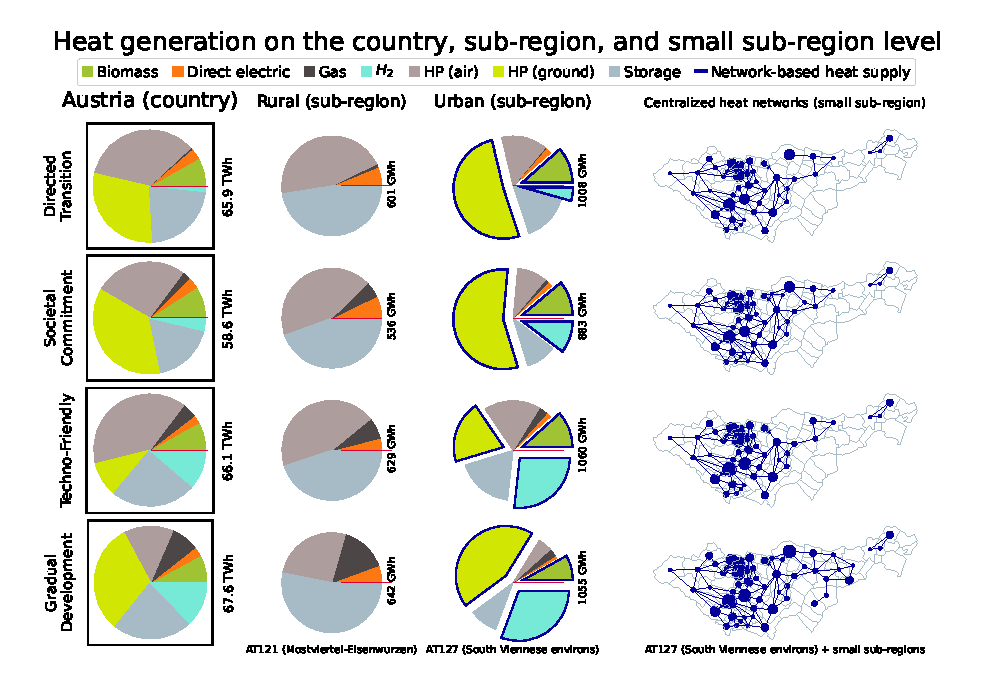
\includegraphics[width=1\linewidth]{figures/4_Results/Spatial_results.eps}
	\caption{Low temperature heat technology generation on different spatial granularity levels for the four different storylines. left: heat technology generation mix on the country level. middle: comparison of technologies supplying the low temperature heat demand in a rural and urban sub-region. right: Centralized heat network topology (size of the points represent the amount of local heat demand supplied by the centralized heat network)}
	\label{fig:res1}
\end{sidewaysfigure}
\newpage
\subsection{Austrian sub-regions with high potentials for centralized low temperature heat supply resulting from aiming the decarbonization}\label{res:3}
As already indicated by Figure \ref{fig:res1}, the results show that there are only a limited number of sub-regions in Austria that have sufficient population and thus heat density to allowing centralized heat supply. Figure \ref{fig:res2} shows a heatmap for centralized heat supply in Austria 2050. Thereby, the spatial granularity corresponds to sub-regions or the NUTS3 level respectively. The corresponding six sub-regions are supplied by the heat networks independent of the storylines. However, the individual quantities of centralized heat supply per sub-region do differ between the storylines (see also exemplarily the heat technology generation mix of the sub-region AT127 in the middle of Figure \ref{fig:res1}). In addition, two comments are essential in this context. Firstly, that Figure \ref{fig:res2} only shows the quantity of centralized heat supply per sub-region. At the same time, heat generation technologies that are not fixed to a central heat distribution network also supply some parts of the heat demand there (see again exemplarily the heat technology generation mix of the sub-region AT127 in the middle of Figure \ref{fig:res1}). Therefore, in those sub-regions in Figure \ref{fig:res2} that are completely white and thus do not have a supply by a centralized heat network, it is shown by the results that the heat demand there is completely covered by technologies that do not require a heat network infrastructure. And secondly, that as expected, the coloured areas are those with the highest population density. This varies between \SI{229}{persons \per \kilo\metre^2} (AT323 - Salzburg and sourroundings) and \SI{5124}{persons \per \kilo\metre^2} (AT130 - Vienna). As indicated in Figure \ref{fig:res2} (orange box), in the following section, the marked sub-regions are further spatially dissaggregated. Subsequently, their heat network topology is analyzed. 

\begin{sidewaysfigure}
	\centering
	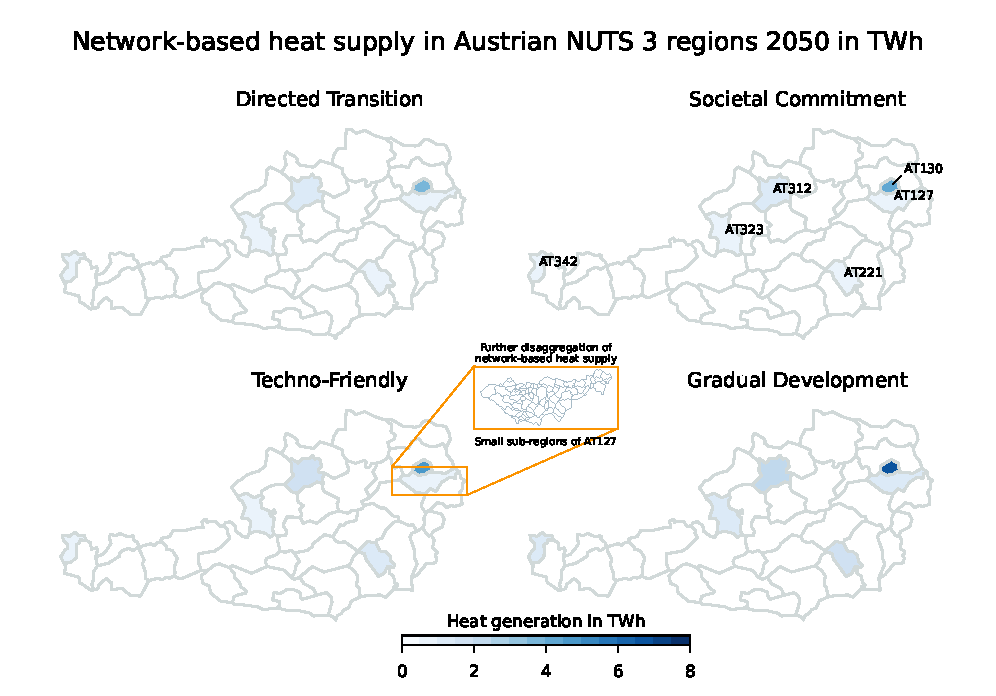
\includegraphics[width=1\linewidth]{figures/4_Results/Heatmap.eps}
	\caption{Centralized low temperature heat supply in Austria 2050. Six sub-regions provide sufficient values of population density to supply parts of the low temperature heat demand by heat networks. The remaining heat demand is supplied by on-site heat technology options. }
	\label{fig:res2}
\end{sidewaysfigure}

\newpage
\subsection{Low temperature heat network topology on the small sub-region level}\label{res:4}
This section analyzes the heat network topology of those regions, that provide sufficient characteristic in terms of population density for centralized heat supply. Figure \ref{fig:res3} shows the boxplot of the benchmark indicator value for the sub-region AT127 (including all small sub-regions). The number of small sub-regions supplied by the centralized heat network is plotted on the horizontal axis. Note that this number decreases from left to right. It becomes visible that by removing small sub-regions, namely iteratively those with the smallest indicator value, the mean indicator value of the entire remaining heat network increases. In addition, the maximum value of the indicator also increases from under 1.64 to over 7.16. In the present example, the number of small sub-regions supplied by the centralized heat network decreases from \SI{75}{} to \SI{47}{} (\SI{-37.3}{\%}). The iteratively reduction of supplied small sub-regions does not necessarily result in a contigous graph. For example, three small sub-regions form a subgraph that is separate from the other network (see upper right in the green box in Figure \ref{fig:res3}).\newline

The results discussed above suggest that reducing the number of small sub-regions supplied by the centralized heat network increase the indicator value and thus the efficiency of the heat network topology. Simultaneously, this also increases the heat density of the supply area. In the following subsection, the obtained heat density values of the heat networks are compared with existing values and today's minimum required values for centralized heat networks.

\begin{sidewaysfigure}
	\centering
	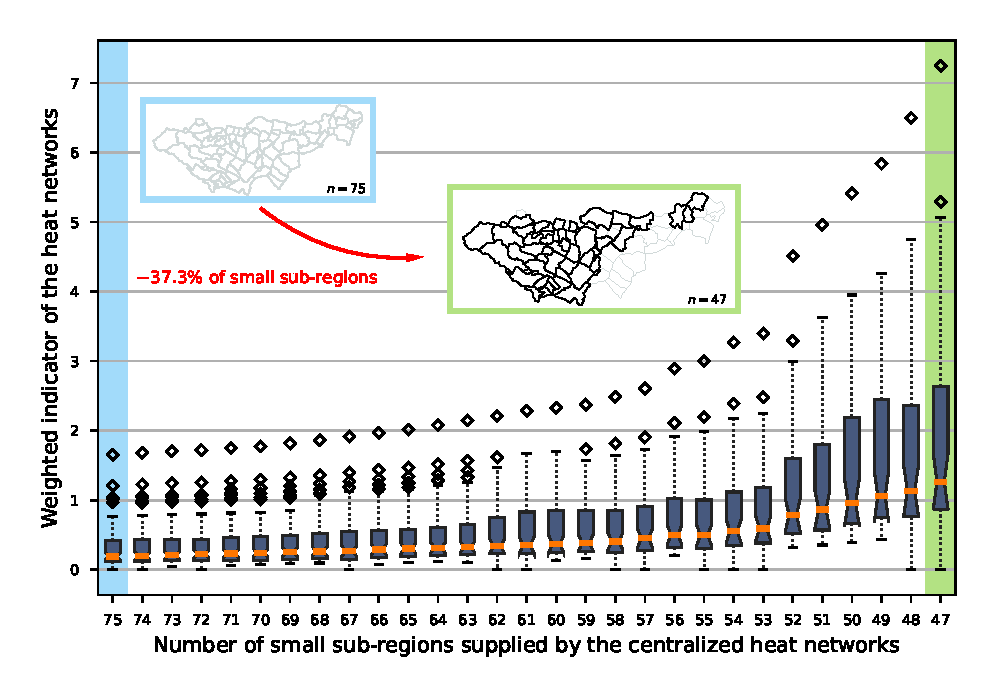
\includegraphics[width=1\linewidth]{figures/4_Results/boxplot.eps}
	\caption{Weighted indicator value of the low temperature heat network at the sub-region AT127 (South Viennese environs) for different numbers of areas supplied by the centralized heat networks.}
	\label{fig:res3}
\end{sidewaysfigure}
\newpage
\subsection{Comparison of existing and future projections of low temperature heat networks using heat and population density}\label{res:5}
This section synthesizes the results in the context of heat density values of centralized heat networks and compares the obtained future projections of sustainable centralized heat supply with current minimum required heat density standards of heat networks. Figure \ref{fig:res4} shows the heat density of low temperature heat networks for different the different proposed downscaling techniques and the four different storylines. The population density is shown on the horizontal axis. The black triangles mark the minimum required heat density for today's centralized heating networks at a connection rate of \SI{90}{\%} in Austria.\footnote{See in this context for example \url{http://www.austrian-heatmap.gv.at/karte/}.} The circles ($\bullet$) mark the default downscaling with only population as criterion. Therefore, the heat density of the sub-regions increases linearly with the population density (see also the zoomed out area in the left subfigure with population density $\leq 150 \frac{persons}{km^2}$). The diamonds ($\blacklozenge$) mark the heat density values obtained by Algorithm 1 (and thus without supply area reduction). As a result, the heat density per sub-region increases (see the zoomed out area in the middle subfigure with population density $\leq 500 \frac{persons}{km^2}$). The stars ($\bigstar$) mark the heat density resulting by Algorithm 2. In order to highlight the effects of the different downscaling techniques, the differences of the resulting heat densities to today's minimum required values is shown for a sub-region by the three green bars for the \textit{Techno-Friendly} storyline. As the comparison of the green bars shows, the difference is again significantly reduced by applying Algorithm 2.

\begin{sidewaysfigure}
	\centering
	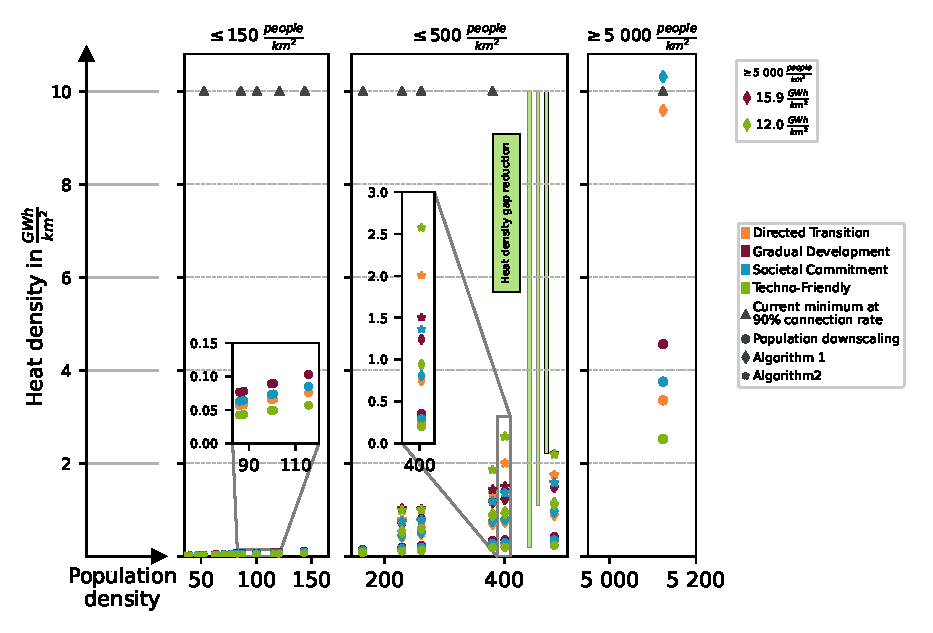
\includegraphics[width=1\linewidth]{figures/4_Results/Heat_density_gap.eps}
	\caption{Heat densities for different population densities, decarbonization storylines, and downscaling techniques. Reducing significantly the gap between today's minimum required heat density (\SI{10}{\frac{GWh}{km^2}} at a connection rate of \SI{90}{\%}) by Algorithm 2 in comparison with default population-based downscaling.}
	\label{fig:res4}
\end{sidewaysfigure}

\newpage
\section{Conclusions and recommendations}\label{conclusions}
\added{The} sustainable energy transition requires methods to bridge the gap between global decarbonization pathways and the \replaced{corresponding}{resulting necessary} measures at local levels. This work emphasizes the development of different downscaling \replaced{techniques}{algorithms}, which we apply to the European heating sector under several \replaced{scenarios}{storylines} in line with the Paris Agreement \added{and its remaining CO\textsubscript{2} budget}. \added{We use the cost-effective European heat supply from the aggregate model GENeSYS-MOD to analyze results at the community level in Austria. The remaining European CO\textsubscript{2} budget (and related CO\textsubscript{2} prices) in line with the 1.5°C climate target is considered by the GENeSYS-MOD results. The downscaling includes the technology-specific infrastructure requirements for the highly efficient usage of heat sources in district heating}.\vspace{0.3cm}

\added{We found that the cost-effective heat supply at the European and national level in 2050 implies that district heating covers parts of the heat demand in four of the thirty-five sub-regions in Austria. Furthermore, the results demonstrate that district heating continues to be picking cherries from beneficial areas (i.e., densely populated with high heat densities) as only some communities of the four mentioned areas are supplied by district heating. Nevertheless, not all district heating networks and supply areas in 2050 reach the heat density required for economic and technical efficiency from today’s techno-economic perspective and industry benchmarks. This heat density gap (mainly driven by a significant reduction of heat demands by building renovation measures) poses a challenge for district heating but can be reduced by the optimal allocation of large-scale heat pump (air) generation into district heating.}\vspace{0.3cm}

\added{We anticipate our work as a starting point for discussing the role of district heating enabling large-scale, highly efficient, and local integration of renewable heat sources such as geothermal, synthetic gas, hydrogen, and waste in sustainable energy systems with decreasing heat demands. Further research should follow on how obtained district heating networks and their heat densities (incl. the generation of large-scale heat pump (air) units) could be returned into more aggregate models, such as GENeSYS-MOD, in the sense of a feedback loop. That allows refining assumptions in the large-scale models, which in turn will increase the plausibility and realism of pathways at the European level.}






\section*{Declaration of interests}
None.
\section*{Declaration of Competing Interest}
The authors report no declarations of interest.
\section*{Acknowledgments}
%This project has received funding from the European Union's Horizon 2020 Research and Innovation Programme under Grant Agreement No. 835896.

\bibliography{mybibfile}
\appendix
\setcounter{table}{0}
\setcounter{figure}{0}
\section{Validation of the downscaled results on the NUTS3 level}
modelle bringen, die ergebnisse zeigen. zumindest message ix ergebnisse. 


\end{document}